\documentclass[11pt,a4paper]{article}
\usepackage[margin=25mm]{geometry}
\usepackage[T1]{fontenc}
\usepackage{lmodern}
\usepackage{graphicx}
\usepackage{float}
\usepackage{enumitem}
\usepackage{hyperref}
\usepackage{xcolor}
\usepackage{caption}
\setlist{nosep,leftmargin=*}
\hypersetup{colorlinks=true,linkcolor=blue,urlcolor=blue}
\setlength{\parskip}{6pt}
\setlength{\parindent}{0pt}
\begin{document}
\begin{titlepage}
\centering
\vspace*{25mm}
{\Large API SECURITY TESTING\\[4mm]}
\rule{\textwidth}{1pt}\\[8mm]
{\huge\bfseries Exploiting an unused API endpoint\\[8mm]}
{\large PortSwigger Web Security Academy Lab Report\\[4mm]}
\vfill
\begin{tabular}{rl}
Platform: & PortSwigger Web Security Academy\\
Tool: & Burp Suite Community Edition\\
Category: & API Testing\\
Status: & Completed\\
\end{tabular}
\vfill
{\small Practical testing performed in an authorized training environment.}
\end{titlepage}
\tableofcontents
\newpage
\section{Objective}
Find and use an API endpoint that is not directly exposed through the normal application interface, then test whether it allows an unintended change to product pricing.
\section{Methodology}
\begin{enumerate}
\item Inspected the application’s requests and responses using Burp Suite while interacting with the shopping functionality.
\item Identified the product price API route: PATCH /api/products/1/price.
\item Tested the endpoint and observed that the server expected the request body to use the application/json content type. A request with an unsupported content type returned HTTP 400 and an explanatory error.
\item Resent the request using Content-Type: application/json and a JSON body setting the price to 0.
\item The server accepted the request and returned HTTP 200 OK with the updated price shown as \$0.00.
\item Added the lightweight leather jacket to the cart and confirmed that its displayed price and order total were \$0.00.
\item Placed the order and confirmed that the lab displayed its successful completion message.
\end{enumerate}
\section{Finding and Result}
The application exposed a price-update API endpoint that could be called directly. The endpoint accepted a client-supplied price of zero and updated the product price, allowing the item to be ordered at no cost in the lab.
\section{Potential Impact}
If a customer can change product prices through an exposed API, this can lead to financial loss, unauthorized price changes and manipulation of orders. The demonstrated impact was limited to the lab environment.
\section{Recommendations}
\begin{itemize}
\item Do not allow ordinary customers to set product prices. Prices should be calculated and controlled by trusted server-side business logic.
\item Enforce role-based authorization for price-management operations.
\item Validate product updates against server-side business rules and trusted data.
\item Ensure the order total is recalculated and verified on the server, rather than trusted from client-controlled values.
\item Monitor and audit changes to product pricing.
\end{itemize}
\section{Evidence}
\begin{figure}[H]
\centering
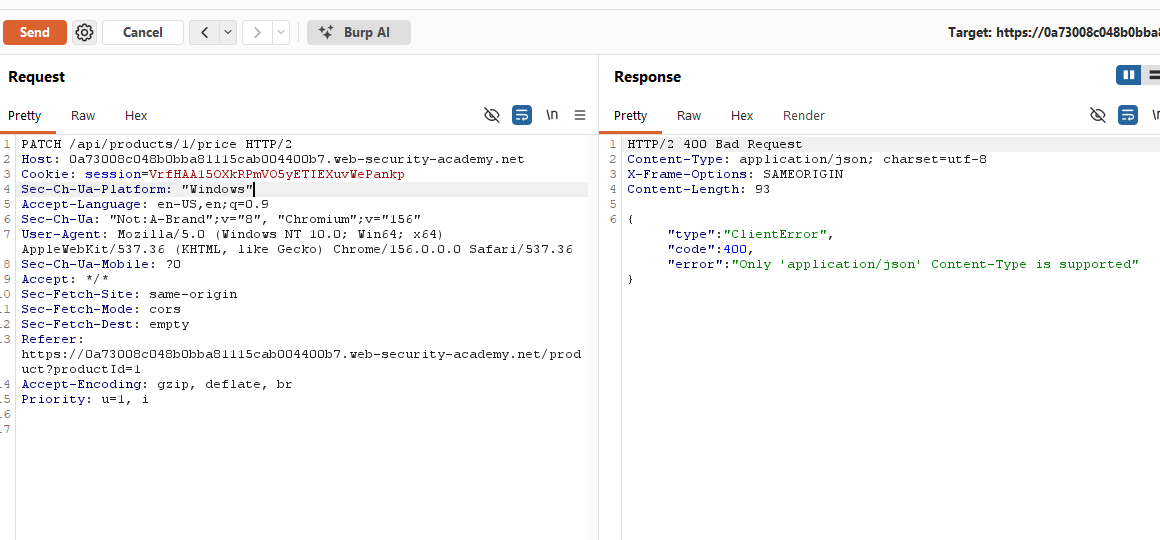
\includegraphics[width=0.96\textwidth,height=0.58\textheight,keepaspectratio]{evidence/testing_allowed_methods.png}
\caption{Burp Suite request and response showing the endpoint and the initial content-type validation error.}
\end{figure}
\begin{figure}[H]
\centering
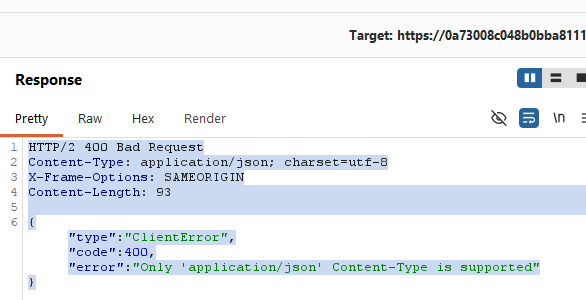
\includegraphics[width=0.96\textwidth,height=0.58\textheight,keepaspectratio]{evidence/content-type.png}
\caption{Server response explaining that application/json is the supported content type.}
\end{figure}
\begin{figure}[H]
\centering
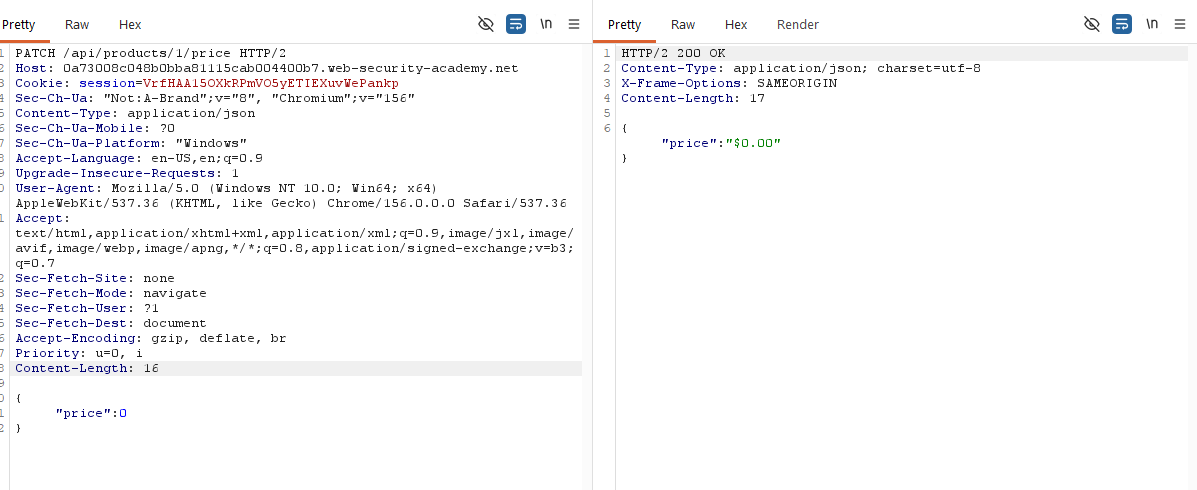
\includegraphics[width=0.96\textwidth,height=0.58\textheight,keepaspectratio]{evidence/price=0.png}
\caption{PATCH request with a JSON price value of zero and the successful response.}
\end{figure}
\begin{figure}[H]
\centering
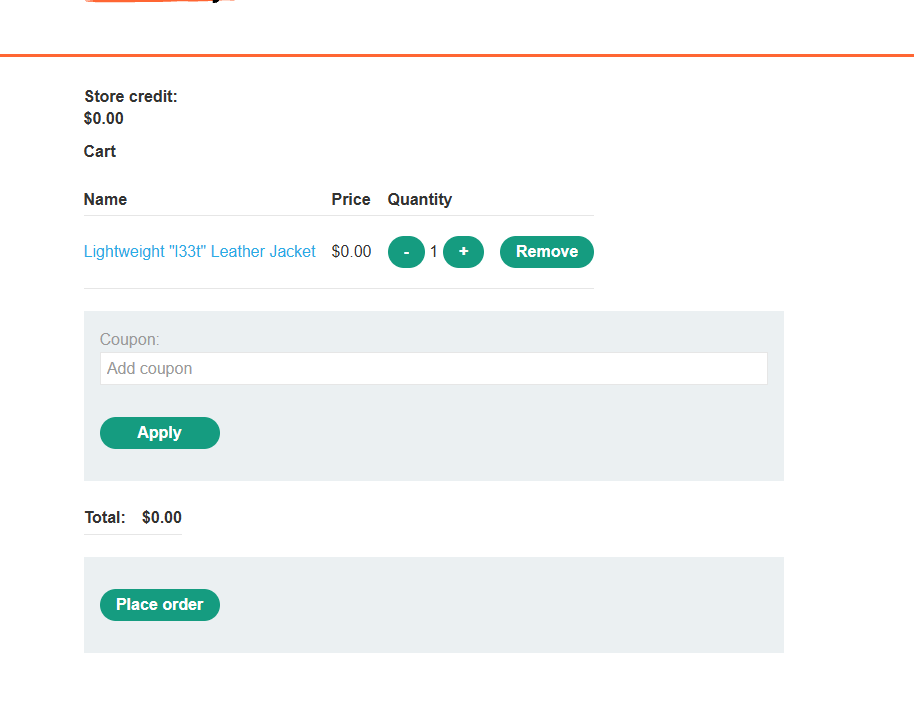
\includegraphics[width=0.96\textwidth,height=0.58\textheight,keepaspectratio]{evidence/jacket_place_order.png}
\caption{Shopping cart showing the jacket and order total at \$0.00.}
\end{figure}
\begin{figure}[H]
\centering
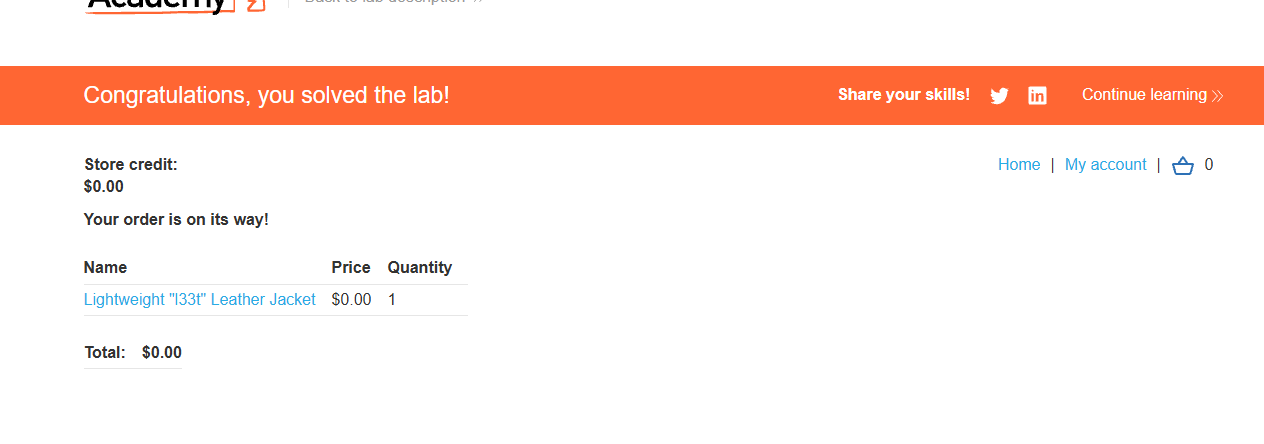
\includegraphics[width=0.96\textwidth,height=0.58\textheight,keepaspectratio]{evidence/solved.png}
\caption{PortSwigger confirmation that the lab was solved.}
\end{figure}
\section{Conclusion}
The exercise showed that an API endpoint can remain callable even when the normal interface does not provide a way to use it. It also demonstrated the business risk of trusting client-supplied values for sensitive operations such as product pricing.
\vfill
{\small Disclaimer: All testing was conducted in the authorized PortSwigger Web Security Academy lab environment.}
\end{document}